% Auto-generated by figures/src/make_captions.py (numbers from figures/src/data). Usage:
% \begin{figure*}[t]\centering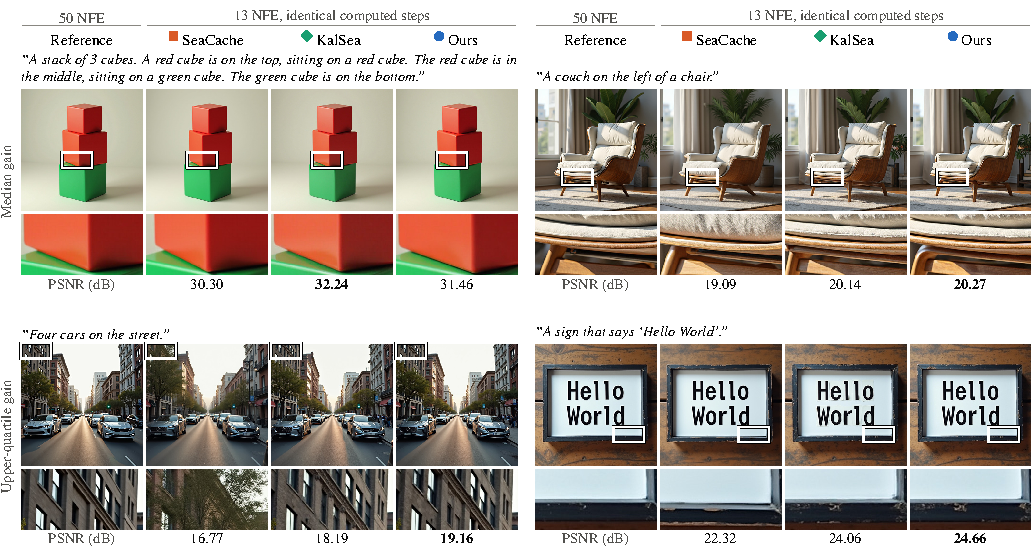
\includegraphics[width=\textwidth]{figures/fig_qualitative.pdf}% Auto-generated by figures/src/make_captions.py (numbers from figures/src/data). Usage:
% \begin{figure*}[t]\centering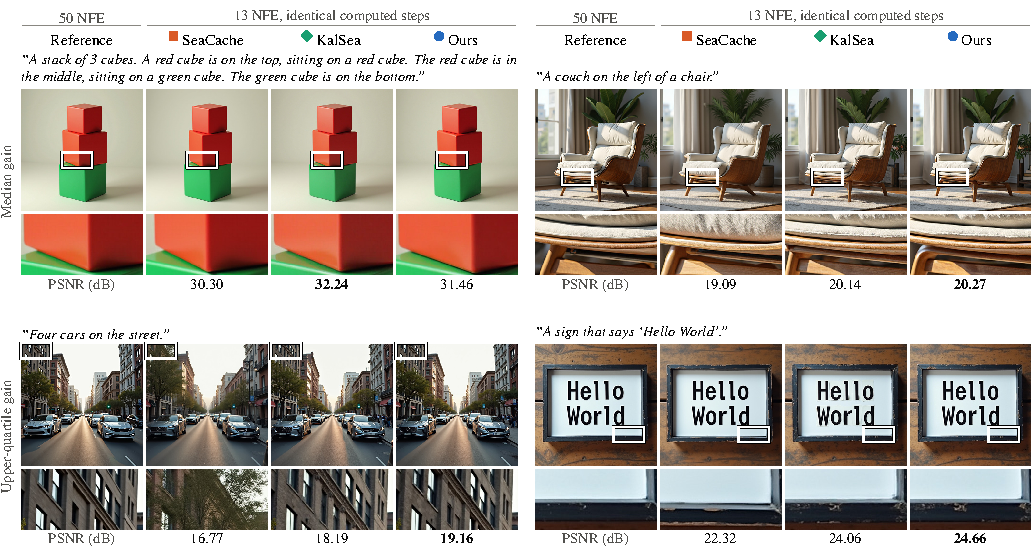
\includegraphics[width=\textwidth]{figures/fig_qualitative.pdf}% Auto-generated by figures/src/make_captions.py (numbers from figures/src/data). Usage:
% \begin{figure*}[t]\centering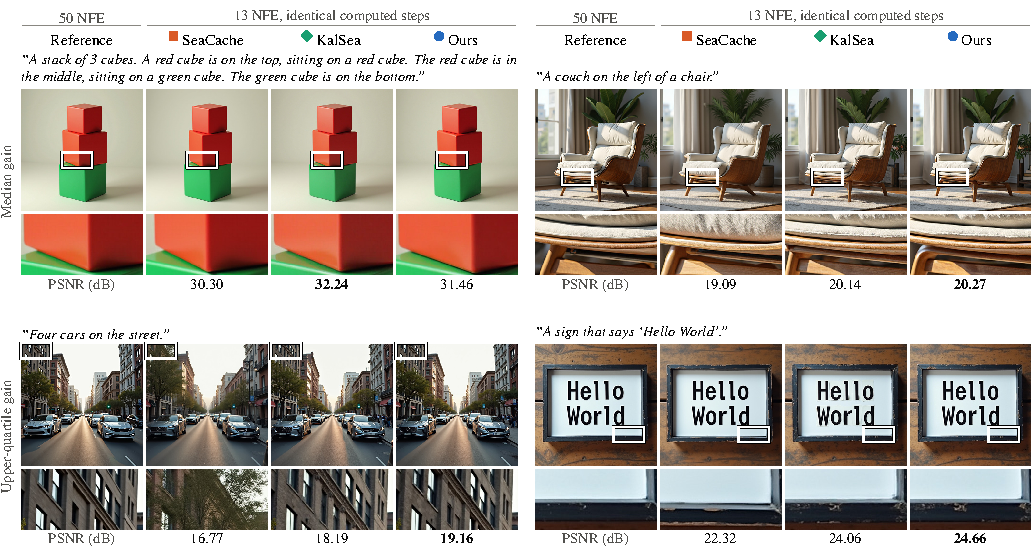
\includegraphics[width=\textwidth]{figures/fig_qualitative.pdf}% Auto-generated by figures/src/make_captions.py (numbers from figures/src/data). Usage:
% \begin{figure*}[t]\centering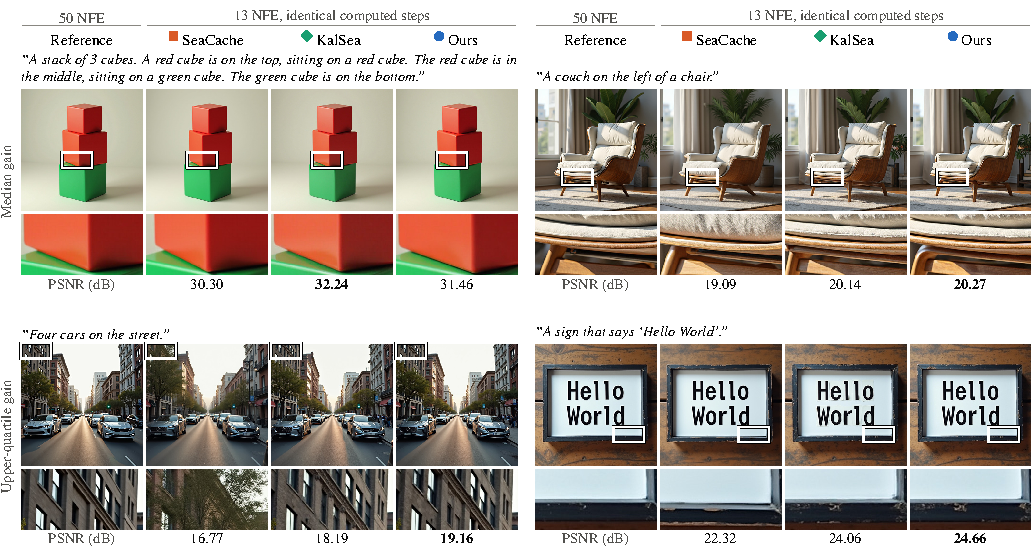
\includegraphics[width=\textwidth]{figures/fig_qualitative.pdf}\input{figures/fig_qualitative_caption}\end{figure*}
\caption{\textbf{Qualitative comparison at 13 \nfe} (\flux, DrawBench, $\delta = 0.6$, $3.8\times$ fewer transformer evaluations than the 50-step reference). The prompts are selected by a fixed rule, not by hand: among the 188 of 200 prompts on which \seacache and \ours computed the identical set of steps, we compute the per-prompt PSNR gain of \ours over \seacache and show the two prompts whose gain is closest to the median (+1.19\,dB; top row) and the two closest to the upper quartile (+2.40\,dB; bottom row). Below each image, a fixed $256\times128$-pixel crop (of $1024\times1024$) is magnified; it is placed where the two accelerated samples differ most (largest mean absolute difference), without looking at the reference. Numbers: PSNR (dB) with respect to the reference, best in bold. Examples near the lower quartile and at the $\approx$21-\nfe budget are in the supplementary material.}
\label{fig:qualitative}
\end{figure*}
\caption{\textbf{Qualitative comparison at 13 \nfe} (\flux, DrawBench, $\delta = 0.6$, $3.8\times$ fewer transformer evaluations than the 50-step reference). The prompts are selected by a fixed rule, not by hand: among the 188 of 200 prompts on which \seacache and \ours computed the identical set of steps, we compute the per-prompt PSNR gain of \ours over \seacache and show the two prompts whose gain is closest to the median (+1.19\,dB; top row) and the two closest to the upper quartile (+2.40\,dB; bottom row). Below each image, a fixed $256\times128$-pixel crop (of $1024\times1024$) is magnified; it is placed where the two accelerated samples differ most (largest mean absolute difference), without looking at the reference. Numbers: PSNR (dB) with respect to the reference, best in bold. Examples near the lower quartile and at the $\approx$21-\nfe budget are in the supplementary material.}
\label{fig:qualitative}
\end{figure*}
\caption{\textbf{Qualitative comparison at 13 \nfe} (\flux, DrawBench, $\delta = 0.6$, $3.8\times$ fewer transformer evaluations than the 50-step reference). The prompts are selected by a fixed rule, not by hand: among the 188 of 200 prompts on which \seacache and \ours computed the identical set of steps, we compute the per-prompt PSNR gain of \ours over \seacache and show the two prompts whose gain is closest to the median (+1.19\,dB; top row) and the two closest to the upper quartile (+2.40\,dB; bottom row). Below each image, a fixed $256\times128$-pixel crop (of $1024\times1024$) is magnified; it is placed where the two accelerated samples differ most (largest mean absolute difference), without looking at the reference. Numbers: PSNR (dB) with respect to the reference, best in bold. Examples near the lower quartile and at the $\approx$21-\nfe budget are in the supplementary material.}
\label{fig:qualitative}
\end{figure*}
\caption{\textbf{Qualitative comparison at 13 \nfe} (\flux, DrawBench, $\delta = 0.6$, $3.8\times$ fewer transformer evaluations than the 50-step reference). The prompts are selected by a fixed rule, not by hand: among the 188 of 200 prompts on which \seacache and \ours computed the identical set of steps, we compute the per-prompt PSNR gain of \ours over \seacache and show the two prompts whose gain is closest to the median (+1.19\,dB; top row) and the two closest to the upper quartile (+2.40\,dB; bottom row). Below each image, a fixed $256\times128$-pixel crop (of $1024\times1024$) is magnified; it is placed where the two accelerated samples differ most (largest mean absolute difference), without looking at the reference. Numbers: PSNR (dB) with respect to the reference, best in bold. Examples near the lower quartile and at the $\approx$21-\nfe budget are in the supplementary material.}
\label{fig:qualitative}
